\documentclass[useAMS,usenatbib]{mn2e}
\usepackage[utf8]{inputenc}
\usepackage{graphicx}
\usepackage{amsmath}
\usepackage{amssymb}
%\usepackage[font={it},labelfont={bf}]{caption}
%\usepackage{units}
\usepackage{times}
\usepackage{color}
\usepackage[usenames,dvipsnames,svgnames,table]{xcolor}
\usepackage{xspace}
\usepackage{subcaption}

\usepackage{fixltx2e} % fixes placing of image positions

\definecolor{customhdrcolor}{rgb}{0.0,0.0,0.0}
\definecolor{customcitecolor}{rgb}{0.0,0.5,0.75}
\definecolor{customlinkcolor}{rgb}{0.0,0.5,0.75}

\usepackage[colorlinks=true,linkcolor=customlinkcolor,urlcolor=customlinkcolor,citecolor=customcitecolor,pdftex]{hyperref}

\ifpdf\pdfinfo{/Title      (WSClean)
               /Author     (A. R. Offringa et al.)
               /Keywords   (instrumentation: interferometers;methods: observational;techniques: interferometric;radio continuum: general)
        }
\else\usepackage{graphics}\fi

\setlength{\pdfpageheight}{\paperheight}
\setlength{\pdfpagewidth}{\paperwidth}

%\newcommand{\editmark}[1]{#1}
%\newcommand{\editmark}[1]{{\color{red}{\textbf{#1}}}}
\newcommand{\degree}{\ensuremath{^{\circ}}\xspace}

% To make Dutch ``tussenvoegsels'' work correctly in Latex such as ``de Bruyn'', we use this command
% It fixes ordering and uppercases.
% In text, it should be written with uppercase, as in ``De Bruyn''
\DeclareRobustCommand{\TUSSEN}[3]{#2}

\title[WSClean: a fast, generic wide-field imager]{WSClean: an implementation of a fast, generic wide-field imager}

\author[A.~R.~Offringa et al.]{A.~R.~Offringa$^{1,2}$\thanks{E-mail:
\url{andre.offringa@anu.edu.au}}, B.~McKinley$^{1,2}$, N.~Hurley-Walker, 
F.~H.~Briggs, \newauthor
J.~Rhee, L.~Feng, D.~Kaplan, A.~R.~Neben, J.~D.~Hughes, MWA commissioning team\newauthor
and GLEAM members where appropriate \& MWA builders list
\\
$^{1}$RSAA, Australian National University, Mt Stromlo Observatory, via Cotter Road, Weston, ACT 2611, Australia \\
$^{2}$ARC Centre of Excellence for All-sky Astrophysics (CAASTRO) \\
}

\begin{document}

\date{Accepted TODO. Received TODO; in original form TODO}
\pagerange{\pageref{firstpage}--\pageref{lastpage}}
\pubyear{2014}

\label{firstpage}
\maketitle

\begin{abstract}
We present our new imager implementation, ``WSClean'', which we find to be an order of magnitude faster than existing implementations, as well as being capable of MWA full-sky imaging at full resolution.
TODO
\end{abstract}

\begin{keywords}
instrumentation: interferometers -- methods: observational -- techniques: interferometric -- radio continuum: general
\end{keywords}

\section{Introduction}

Observations from non-coplanar interferometric radio telescopes that image large fractions of the sky at once can not be imaged with simple imagers that are based on a two-dimensional Fast Fourier Transformation (FFT). Instead, the imaging algorithm needs to account for the ``w-term'' during inversion, which is the term that describes the deviation of the array from a perfect plane \citep{perley-noncoplanar-arrays}. This deviation is amplified for telescopes with wide field of view, making this especially an issue for low-frequency telescopes, that by nature are wide-field instruments.

There are several methods to deal with the w-term during imaging: facetting \citep{facetting-cornwell}, a three-dimensional Fourier transform \citep{perley-noncoplanar-arrays}, w-projection \citep{wprojection-cornwell}, w-stacking\footnote{TODO when/where was this first mentioned in literature?} \citep{widefield-imaging-ska-cornwell} and w-snapshots \citep{widefield-imaging-ska-cornwell}. The w-snapshots algorithm is a hybrid between snapshot imaging and one of the other w-term correcting techniques, most efficiently w-projection or w-stacking.

New generation of wide-field observatories are producing data sets that are orders of magnitude larger than before. Examples of such telescopes include the Murchison Widefield Array (MWA, \citealt{mwa}), the upgraded Jansky Very Large Array (JVLA) and the Low-Frequency Array (LOFAR, \citealt{lofar-2013}). At the MWA, some of the data is reduced with the w-projection algorithm implementation of the Common Astronomy Software Applications (CASA, \citealt{casa}). This is an attractive option because of its many features, high quality and free availability. However, at the MWA we have seen that imaging a 2-min snapshot observation at low-elevation can take up to tens of hours with CASA's w-projection algorithm. Another option for reducing MWA data is the Real-Time System (RTS), which has been designed as an efficient calibrating and imaging pipeline specifically for MWA data \citep{rts-mwa}. It can use GPUs for improving efficiency, and uses a w-projection kernel during imaging to correct for the w-term. The kernel can be kept small, because the data is processed in snapshots that have been phase-centered to Zenith. The RTS can not perform deconvolution as of yet.

To reach high dynamic ranges, it can be necessary to deal with direction-dependent effects (DDEs). This is especially true for widefield telescopes. One way to handle DDEs is by using the a-projection technique, which convolves the data during gridding with a kernel that corrects the DDEs \citep{aprojection-2008}.
One such DDE is the effect of the ionosphere. For the MWA it can be assumed that the ionosphere has the same effect on all tiles, because the maximum baseline length is relatively small (2.9~km) and smaller than the typical size of ionospheric structure (TODO cite). This is not the case for LOFAR, making it necessary to correct the direction-dependent ionospheric effects per station before gridding the data. The \texttt{awimager} has been written to perform these corrections, and uses a hybrid of a-projection, w-projection and w-stacking \citep{awimager-2013}.

Once the Square-Kilometre Array (SKA) begins its operation, the required computational power for wide-field imaging will become an even bigger challenge. In \citet{widefield-imaging-ska-cornwell}, it is shown that in theory the w-snapshots algorithm is the most efficient approach for the SKA.

In this article, we present a new implementation of a generic wide-field imager that is significantly faster than CASA's w-projection implementation. To obtain the increase in speed, the implementation uses the w-stacking method for correcting the w-terms, optionally combined with w-snapshot imaging. We named the new imager ``WSClean'', as an abbreviation for ``W-Stacking Clean''. This work improves the field of wide-field imaging in the following ways:
\begin{itemize}
 \item The performance of w-stacking is compared to w-projection.
 \item Parameters that affect the w-snapshots algorithm are analysed.
 \item Details are described of how to efficiently implement the w-stacking and w-snapshots algorithms.
 \item A new implementation is released, which we believe to be the fastest generic widefield imager available.
\end{itemize}

The w-stacking algorithm is described in Sect.~\ref{sec:wstacking}. Details of implementing the w-stacking and w-snapshots algorithms are described in Sect.~\ref{sec:implementation}. The performance and accuracy will be analysed in Sect.~\ref{sec:analysis}.

\section{The w-stacking technique} \label{sec:wstacking}
In this section, we will describe the w-stacking algorithm from a mathematical point of view.

An interferometer samples the complex visibility function
\begin{align}\notag
V(u,v,w) = & \iint \frac{A(l,m) I(l,m)}{\sqrt{1-l^2-m^2}} \cdot \\ \label{eq:visibility-function}
& e^{-2\pi i \left(ul + vm + w(\sqrt{1-l^2-m^2}-1)\right)} dl dm,
\end{align}
where $u,v,w$ is a baseline coordinate in the coordinate system of the array, $A$ is the primary-beam function, $I$ is the sky function and $l,m$ are cosine sky coordinates. We will use $I'(l,m)$ to denote the sky function before primary-beam correction, $I'(l,m)=A(l,m)I(l,m)$. We will not discuss calibration, but assume $V$ has been calibrated before imaging. In the case of a polarized measurement, the symbols $V$, $A$ and $I$ are $2\times 2$ Jones matrices, but without loss of generality we will ignore polarization and treat inversion as a scalar problem. Imaging consists of inverting Eq.~\eqref{eq:visibility-function}, i.e., to find $I'$ from $V$.

For small field of views, the term $\sqrt{1-l^2-m^2}$ is approximately of unit size, making Eq.~\eqref{eq:visibility-function} approximate an ordinary 2-dimensional Fourier transform, which can be inverted with an inverse Fast Fourier Transform (FFT). A common rule is that this is valid when
\begin{equation}\label{eq:when-2d-is-valid}
\forall w,l,m: w\left(\sqrt{1-l^2-m^2}-1\right) \ll 1.
\end{equation}

To derive the w-stacking technique, Eq.~\eqref{eq:visibility-function} is rewritten to
\begin{align}\notag
V(u,v,w) = & \iint \frac{I'(l,m) e^{-2\pi i w(\sqrt{1-l^2-m^2}-1)}}{\sqrt{1-l^2-m^2}} \cdot \\ \notag
& e^{-2\pi i \left(ul + vm\right)} dl dm.
\end{align}
This is an ordinary two-dimensional Fourier transform going from $u,v$ space to $l,m$ space, and can be inverted to get:
% Intermediate step:
%\begin{align}\notag
%\frac{I'(l,m) e^{-2\pi i w(\sqrt{1-l^2-m^2}-1)}}{\sqrt{1-l^2-m^2}} = & \iint V(u,v,w) \cdot \\ \notag
%& e^{-2\pi i \left(ul + vm\right)} du dv,
%\end{align}
%which can be rewritten to
\begin{align}\notag
\frac{I'(l,m)}{\sqrt{1-l^2-m^2}} = & e^{2\pi i w(\sqrt{1-l^2-m^2}-1)} \iint V(u,v,w) \cdot \\ \notag
& e^{2\pi i \left(ul + vm\right)} du dv.
\end{align}
Integrating both sides over $w_0$ to $w_e$, the minimum and maximum value of $w$, results in
\begin{align}\notag
\frac{I'(l,m)\left(w_e - w_0\right)}{\sqrt{1-l^2-m^2}} = \int\limits_{w_0}^{w_e} e^{2\pi i w(\sqrt{1-l^2-m^2}-1)} \cdot \\ \label{eq:wstacking}
\iint V(u,v,w)  e^{2\pi i \left(ul + vm\right)} du dv dw.
\end{align}
The final step is to make the $u,v,w$ parameters discrete, so that the integration over $u$ and $v$ can become an inverse FFT and the integration over $w$ becomes a summation. This shows that the sky function can be reconstructed by i)~grid samples with equal $w$-value on a uniform grid; ii)~calculating the inverse FFT; iii)~apply the direction dependent phaseshift $e^{2\pi i w(\sqrt{1-l^2-m^2}-1)}$; iv)~repeat this for all $w$-values and add the results together; v)~apply the final scaling.

In practice, the final scaling will be different from $\left(w_e - w_0\right)/\sqrt{1-l^2-m^2}$ suggested by Eq.~\eqref{eq:wstacking}, because the individual $w$-layers will not be completely filled with samples. Therefore, the number of added samples and their weight have to be taken into account. Additionally, it might be required to divide out the effect of a possible convolution kernel, the primary beam and correct for other direction dependent effects. In XX, YY, LL or RR polarizations, a correlated baseline is the complex conjugate of the reversed baseline, and the relation $V(u,v,w)=\overline{V(-u,-v,-w)}$ holds. The right-hand side of Eq.\eqref{eq:wstacking} with only positive $w$-value samples then becomes the complex conjugate of the one with only negative $w$-values samples. In this case we can therefore calculate the image for $w<0$ from the image with $w>0$. That allows us to set $w_0$ to the minimum absolute $w$-value, which requires at least two times less layers. In any case, the input to the two-dimensional inverse FFT is not generally an Hermitian-symmetric function, and hence is always performed as a complex-to-complex transform. 

The inverse of imaging, i.e., to calculate the visibility from a model image, can be done by reversing the $w$-stacking algorithm: i)~inverse scale the image; ii)~copy the image to several layers; iii)~inverse apply the direction-dependent phaseshift for each layer; iv)~FFT each layer; and v)~sample a required visibility from the correct $w$-layer. We will refer to this operation as prediction.

\subsection{Discretization of w} \label{sec:gridding-w}
\begin{figure}
\begin{center}
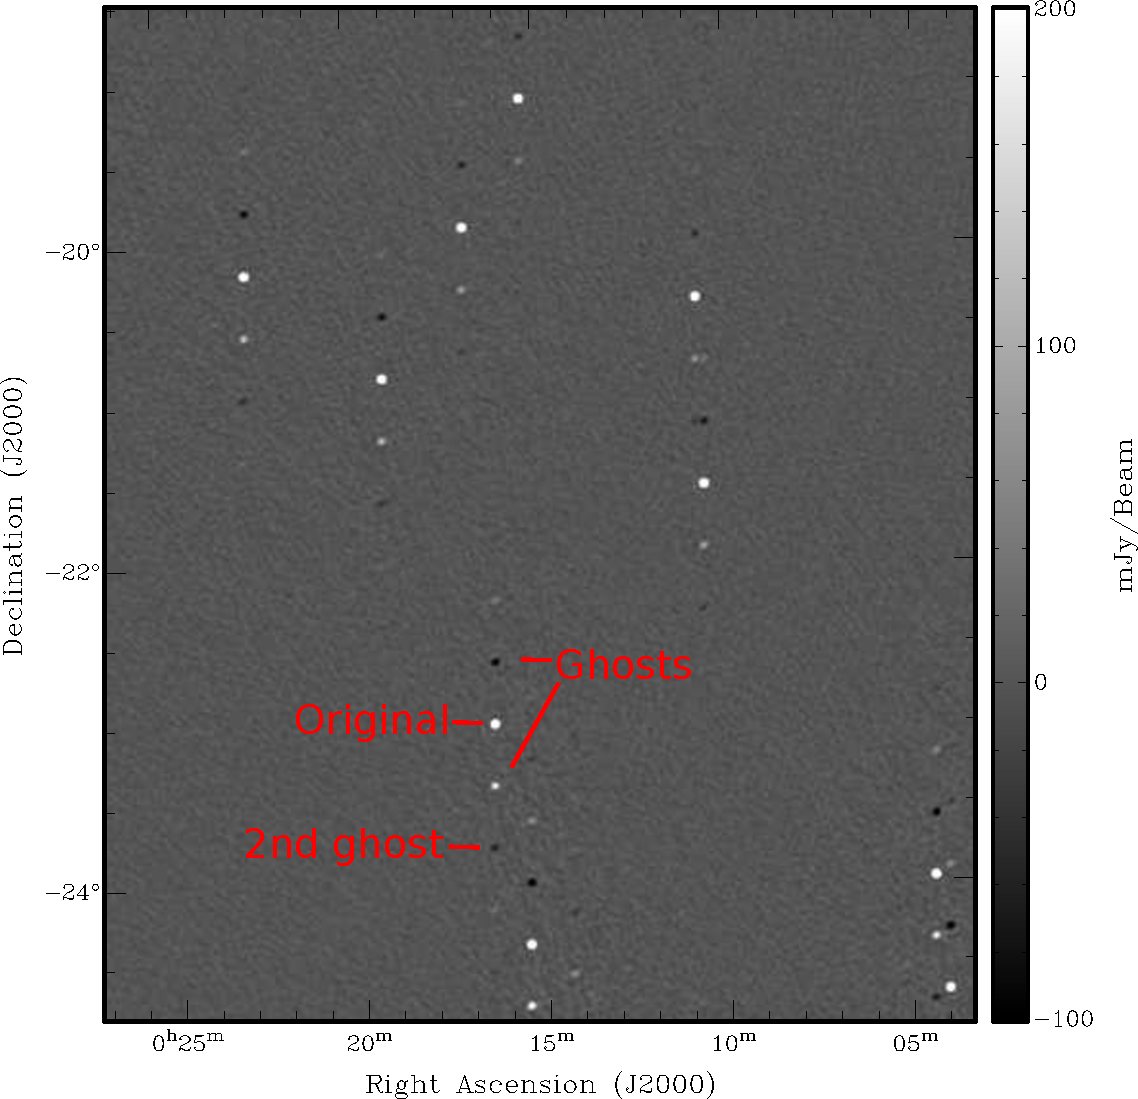
\includegraphics[width=8cm]{img/aliasing-example-annotated}
\caption{Aliasing artefacts caused by insufficient $w$-layers in a simulated field. WSClean was set to use 12 $w$-layers. The centre of the image is at 10\degree zenith angle, which would normally require $\sim195$ $w$-layers. Original sources are 1~Jy, ghost sources are approximately 20\%. Each source produces two ghost sources, but because they re-appear after a major cleaning cycle, they are eventually cleaned and produce more ghost sources. }
\label{fig:aliasing-example}
\end{center}
\end{figure}
While the discretization of $u$ and $v$ is similar to conventional imaging, the discretization of $w$ defines the number of w-layers that need to be processed. For this, one can use a rule similar to \eqref{eq:when-2d-is-valid}, and make sure that the phase difference for two subsequent discretized $w$-values, $w_A$ and $w_B$,  is less than one radian. This results in the constraint
\begin{equation} \label{eq:minimum-w-distance}
\left|\left(w_A - w_B\right) 2\pi (\sqrt{1-l^2-m^2}-1)\right| \ll 1.
\end{equation}
This suggest that a uniform discretization in $w$ is optimal TODO in contrast to some article? -- could be explained by having more samples at smaller $w$s. From Eq.~\eqref{eq:minimum-w-distance}, the required number of layers can be derived and is given by
\begin{equation} \label{eq:nwlayers-bound}
 N_\textrm{wlayers} \gg 2\pi \left(w_e - w_0\right) \max_{l,m} \left(1 - \sqrt{1-l^2-m^2}\right).
\end{equation}
Actual values for the right-hand side can differ a lot. The value of $w_e - w_0$ is influenced by the coplanarity of the array, the zenith angle and the wavelength, while the value of the $\max_{l,m}$ term is influenced by the angular size of the image. For the MWA, a typical value of $w_e - w_0$ is $\sim 10$ at zenith, but is already $\sim 400$ at a zenith angle of $30^{\circ}$. [TODO table of arrays with $w$ values at zenith/more angles/more freq?] For a typical full-field-of-view image of a MWA observation of $3072\times 3072$ pixels of $0.75''$ size, the $\max_{l,m}$ term is $0.68$. This implies that, in the case of the MWA, tens of $w$-layers are required at zenith and hundreds at lower elevations. The number of $w$-layers has a large effect on the performance of the $w$-stacking algorithm, and will be discussed further in the next sections.

Using too few $w$-layers results in decorrelation of off-axis sources in the longer baselines. Additionally, $w$-aliasing errors can cause ghost sources in the image. An (extreme) example of this effect is shown in Fig.~\ref{fig:aliasing-example}. When Cotton-Schwab cleaning includes prediction with too few $w$-layers, incorrect values will be subtracted from the visibilities even when no aliased sources are cleaned during minor iterations. Therefore, accurate prediction is more important than accurate imaging, because aliasing artefacts are attenuated by cleaning as long as the model is subtracted accurately. Possible ways to allow less $w$-layers during imaging is by predicting with more $w$-layers or a direct Fourier transform. We have not looked into these options yet.

\subsection{Time complexity of w-stacking} \label{sec:time-complexity}
It is useful to analyse the time complexity of w-stacking and compare it with w-projection, to understand which algorithm performs better in a given situation. We will use the following symbols: $N_\textrm{wlay}$ is the number of w-layers for w-stacking, $N_\textrm{pix}$ is the number of pixels in the image along each dimension, $N_\textrm{vis}$ is the number of visibilities and $N_\textrm{kern}$ is the size of the antialiasing kernel (see \S\ref{sec:gridding}), $N_\textrm{wkern}$ is the size of the w-kernel for w-projection, $w_e$ is the maximum $w$ value and $\alpha_\textrm{FOV}$ is the imaging field of view.

\begin{table}
 \caption{Scaling of the computational cost for various imaging steps} \label{tbl:computational-cost-per-operation}
 \begin{tabular}{lll}
   \textbf{Operation} & \textbf{W-stacking} & \textbf{W-projection} \\
   \hline\hline
   Fourier transform(s) & $N_\textrm{wlay} N^2_\textrm{pix} \log N_\textrm{pix}$ & $N^2_\textrm{pix} \log N_\textrm{pix}$ \\
   W-term corrections   & $N_\textrm{wlay} N^2_\textrm{pix}$ & $N_\textrm{vis} N^2_\textrm{wkern}$ \\
   Gridding & $N_\textrm{vis}N^2_\textrm{kern}$ & $N_\textrm{vis} N_\textrm{kern}^2$ \\
   \hline\hline
 \end{tabular}
\end{table}

Table~\ref{tbl:computational-cost-per-operation} shows how the computational costs scale for the operations that dominate the imaging in the w-stacking and w-projection algorithms. For comparison, we can assume the gridding kernel adds a constant term and the terms $N_\textrm{wlay}$ and $N_\textrm{wkern}$ follow approximately $w_e \sin \alpha_\textrm{FOV}$. The time complexity for w-stacking is then given by
\begin{equation}
\textrm{TC}_\textrm{wstacking}=\mathcal{O}\left(N^2_\textrm{pix} \log N_\textrm{pix} w_e \sin \alpha_\textrm{FOV}+ N_\textrm{vis} \right),
\end{equation}
and for $w$-projection it is
\begin{equation}
\textrm{TC}_\textrm{wprojection}=\mathcal{O}\left(N^2_\textrm{pix} \log N_\textrm{pix} + N_\textrm{vis} w_e^2 \sin^2 \alpha_\textrm{FOV}\right).
\end{equation}
From these bounds it can be concluded that in the limiting behaviour, the $w$-stacking method will be faster when the gridding of the visibilities is the dominating cost of the algorithm. The $w$-projection algorithm will be faster when the inverse FFTs are dominating. In Sect.~\ref{sec:analysis} we will determine which method is faster in practice for different parameters.

\section{The WSClean imager implementation} \label{sec:implementation}
With the purpose of testing new algorithms for the imaging of MWA data, we have written a new imager around the $w$-stacking algorithm. The imager is not specialized for the MWA, and has been succesfully used for other telescopes (TODO menton more).

The new imager, called ``WSClean'', is written in the C++ language. It reads visibilities from CASA measurement sets and writes output images to Flexible Image Transport System (FITS) files. Several steps are multi-threaded: reading and writing; gridding from and to different $w$-layers; performing the Fast Fourier transforms; and H\"ogbom Clean iterations (peak-finding and image subtraction, \citealt{hogbom-clean}). For the latter, intrinsics are used as well. Because of these optimizations, minor Cleaning iterations with an image size of $3072\times3072$ are performed at a rate of hundreds per second. This is fast enough to make the Clark Clean optimization \citep{clark-clean}, which consists of considering only a subset of pixels with a reduced PSF, less relevant. However, the PSF varies for imaging with non-zero $w$-values, and subtracting a constant PSF in image space leads to inaccuracies. After a number of minor iterations, it is therefore beneficial to invert the model back to the visibilities via prediction, and subtract the model directly from the visibilities \citep{wprojection-cornwell}. This is similar to the Cotton-Schwab cleaning method \citep{cotton-schwab-clean}.

It will not be possible to store all $w$-layers in memory when creating large images or when many $w$-layers are used. For example, our 32-GB test machine can store 227 $w$-layers of $3072\times3072$ in memory. In more demanding imaging configurations, the implementation performs several passes over the measurement set and will grid a subset of $w$-layers in each pass.

\subsection{Full-sky imaging}
For low-frequency telescopes, it can be of interest to do full-sky imaging. In the case of MWA, the tile beam can have strong sidelobes at a distance of more than 90\degree from the pointing centre. Imaging these sidelobes might be relevant because it might either be scientifically interesting (e.g. when searching for transients), or be useful for self-calibration or full-sky deconvolution. For example, the latter is useful when a strong source in a sidelobe affects the sensitivity near the pointing centre.

To efficiently image the full sky, an observation is split into short snapshots, their phase centre is changed to zenith and subsequently a suitable area is imaged. Depending on desired resolution and dynamic range, this might require very large images. To make an image at the MWA resolution, the image needs to have approximately 10K pixels in width and height. The $w$-values will be very small at zenith, because at zenith only the vertical offsets of the antennas will contribute to the $w$-value. For the MWA, the maximum height difference between tiles is $8.5$m. The MWA tiles are in fact on a slight slope, and by fitting a plane to the antennas and changing the phase centre towards the normal of that plane, the maximum $w$-value decreases to $5.5\textrm{m} / \lambda$. In the following sections, when discussing the MWA zenith direction we are referring to this optimal $w$-direction.

\subsection{W-snapshots} \label{sec:snapshot-imaging}
\begin{figure*}
\begin{center}
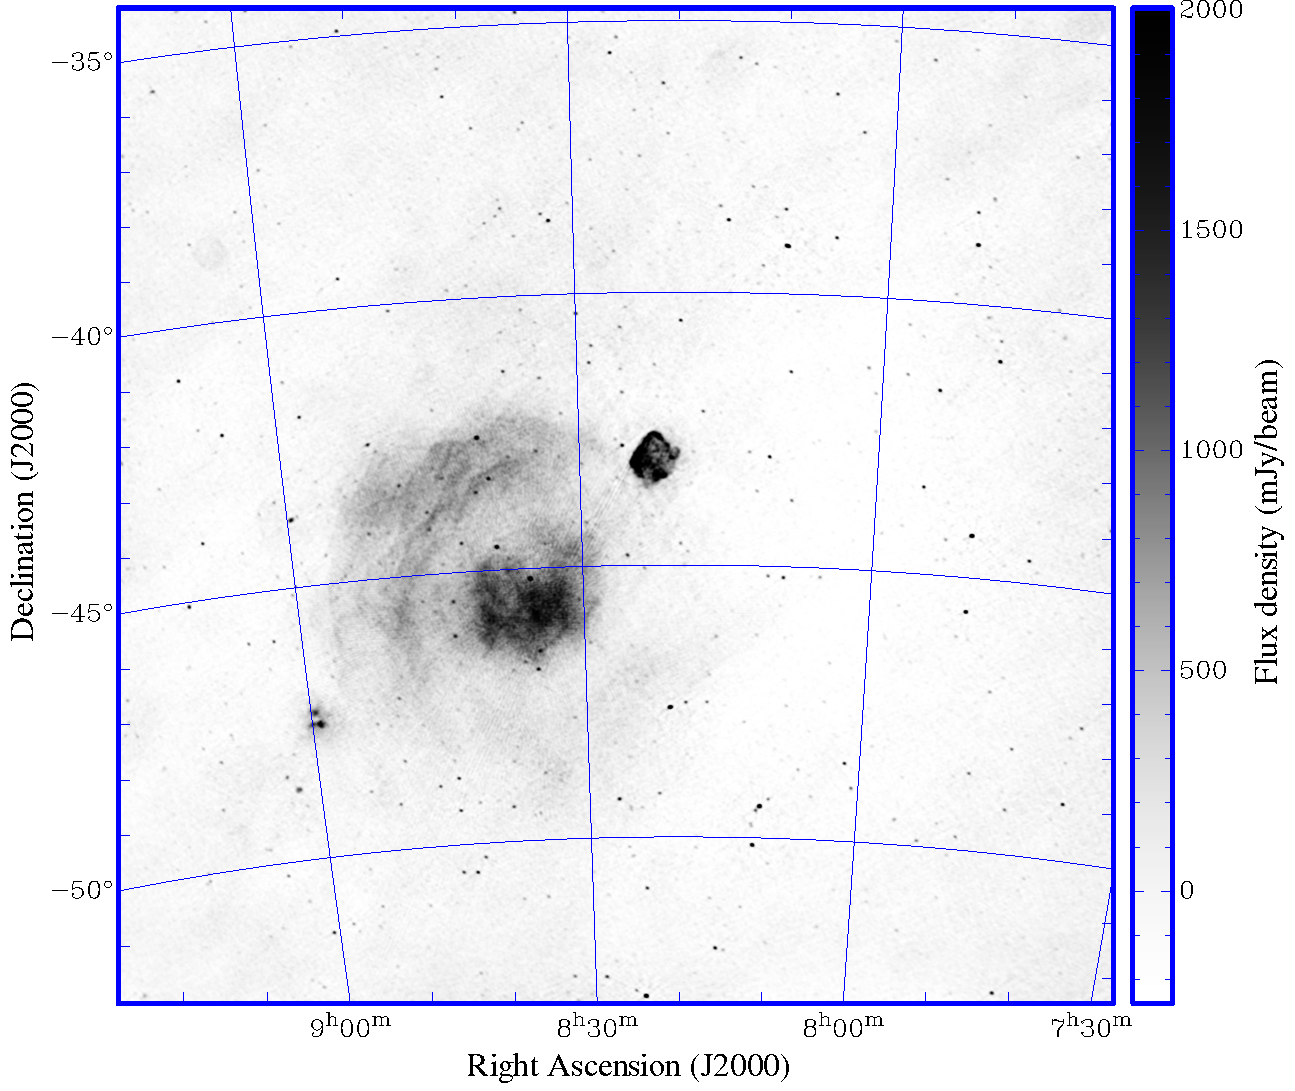
\includegraphics[width=8cm]{img/vela-normal-projection}
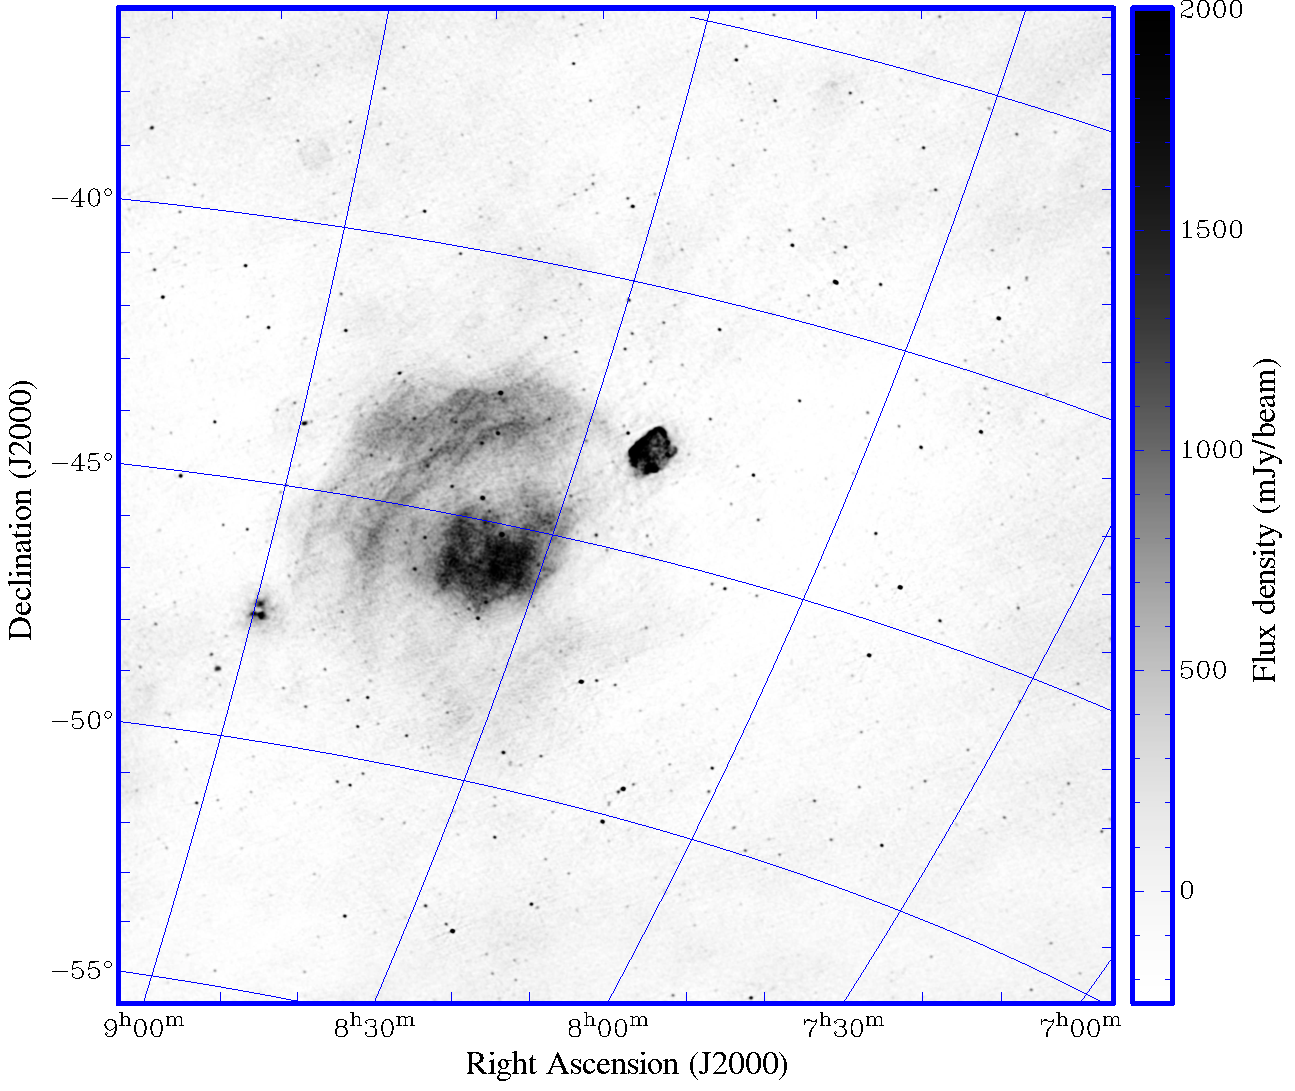
\includegraphics[width=8cm]{img/vela-zenith-projection}
\caption{13-min MWA observation of supernova remnants Vela and Puppis A. Left: normal projection centred on Puppis A, right: phase-rotated to zenith to reduce $w$-values, recentred on Puppis A during imaging. Both Stokes-I images have been made with WSClean using the Cotton-Schwab clean algorithm. No beam correction was applied. TODO time difference and more discussion, replace with deeper images.}
\label{fig:vela-projection-example}
\end{center}
\end{figure*}
As discussed, all-sky snapshot imaging with zenith as phase centre is quite efficient. However, if one is not interested in imaging the whole sky, and the direction of interest is far from zenith, the computational overhead of making all-sky images is undesirable.

Instead of imaging the whole sky, the image can be recentred from $(l,m)$ to $(\hat{l},\hat{m})=(l+\Delta l,m+\Delta m)$ by performing the substitution $(l,m)\leftarrow(\hat{l},\hat{m})$ in Eq.~\eqref{eq:wstacking}:
%When the Fourier transform is performed, the $w$ term has been corrected (either by w-stacking or by w-projection). Therefore, if $U(u, v)$ is the input to the 2-dimensional Fourier transform, the transform is described by
\begin{align}\notag
\frac{I'(\hat{l}, \hat{m})\left(w_e - w_0\right)}{\sqrt{1-\hat{l}^2-\hat{m}^2}} = \int\limits_{w_0}^{w_e} e^{2\pi i w(\sqrt{1-\hat{l}^2-\hat{m}^2}-1)} \cdot \\
\iint e^{2 \pi i \left(u\Delta l + v\Delta m\right)} V(u,v,w) e^{2\pi i \left(ul + vm\right)} du dv dw.
\end{align}
In words, recentering an image involves accounting for the position shift during the $w$-correction and final scaling, and shifting the visibilities in phase by multiplication with $e^{2 \pi i \left(u\Delta l + v\Delta m\right)}$ prior to the imaging. This essentially is a method of implementing the $w$-snapshots algorithm as described by \citet{widefield-imaging-ska-cornwell}. By doing the inverse corrections during prediction, such a shifted visibility set can be cleaned with Cotton-Schwab iterations similar to a non-shifted set.

A recentred image is in the projection of the zenith tangent plane, and will need an additional regridding step before multiple snapshots can be added together. A recentred image can be stored in a Flexible Image Transport System (FITS) file, which allows setting the centre of tangent projection with the \texttt{CRPIXi} keyword \citep{wcs-in-fits}. Common viewers such as Kvis and DS9 support such FITS files and display their coordinates correctly. An example of the difference in projection is given in Fig.~\ref{fig:vela-projection-example}, which displays a 13~min MWA observation imaged with WSClean. Cleaning an image that is in a different projection yields slightly different results, but qualitativily the two images are clearly of equal accuracy.

Another method to shift an image is by using the periodicity of the FFT function. Since sources outside the field of view will be aliased back into the field, the image can be transformed to have the alias in the centre. This complicates gridding during imaging, because the antialiasing kernel needs to have a pass-band shape instead of a low-pass shape. Therefore, we chose to implement the former method.

\subsection{Gridding} \label{sec:gridding}
A gridding convolution kernel improves the accuracy of gridding in $uv$-space. A common kernel function is a windowed sinc function, which acts as a low-pass filter. This decreases the flux of sources outside the field of view, and thus helps to attenuate aliased ghost sources and sidelobes that arise because of the assumed periodicity during the inverse FFT \citep{post-correlation-filtering}. By supersampling, a convolution kernel also makes it possible to place samples more accurately at their $uv$ position, thereby lowering decorrelation.

The prolate spheroidal wave function (PSWF) is generally considered to be the optimal windowing function for gridding \citep{fourier-kernel-selection-1991}. CASA convolves samples with a PSWF of 7 pixels total width during gridding. When using a variable kernel size, a PSWF is quite complicated and computational expensive to calculate. WSClean currently uses a Kaiser-Bessel (KB) window function, which is easy and fast to compute, and is a good approximation for the PSWF \citep{fourier-kernel-selection-1991}. After some benchmarks (see Appendix~\ref{sec:gridding-appendix}) we found that 7 pixels is a good compromise between performance and accuracy, and selected this as the default for WSClean.

\section{Analysis} \label{sec:analysis}
We will now analyse the performance and accuracy of our implementation, and compare it with the w-projection implementation in CASA. For the analysis, we use imaging parameters which are common for MWA Imaging. When a specific parameter value is not mentioned, the settings from Table~\ref{tbl:default-parameters} are used. The number of $w$-projection planes in w-projection is kept equal to the number of $w$-layers in w-stacking, and is set to the right hand side of Eq.~\eqref{eq:nwlayers-bound}. This yields 195 $w$-planes/layers at 10\degree zenith angle. Some configurations with high $w$-values fail to image with CASA, presumably because the $w$-kernels become to large.

The used software version of CASA is ``stable release 42.0, revision 26465'', which was released September 2013. It includes performance improvements to the \texttt{clean} task which have recently been made. For WSClean, the latest version as of February 2014 was used. The tests were run on a high-end desktop, with a 3.20-GHz Intel Core i7-3930K processor with 6 cores and 32 GB of memory. The data are stored on a multi-disk array with 5 spinning hard disks, which has a combined read rate of about 450 MB/s.
\begin{table}%
\caption{Parameter values used during benchmarks, unless otherwise mentioned.} \label{tbl:default-parameters}%
\begin{center}\begin{tabular}{rl}%
\hline
Array & MWA 128T \\
Image size & $3072 \times 3072$ \\
Angular resolution & $0.72'$ \\
Number of visibilities & $3.5 \times 10^8$ \\
Time resolution & 2~s \\
Frequency resolution & 40~kHz \\
Observation duration & 112 s\\
Bandwidth & 30.72 MHz (768 channels)\\
Central frequency & 182 MHz \\
Zenith angle at phase centre & 10\degree \\
Max $w$-value for phase centre & 172 $\lambda$ (283 m) \\
Nr. polarizations in set & 4 \\
Imaged polarization & XX \\
Imaging mode & Multi-frequency synthesis \\
Weighting & uniform \\
Data size & 18 GB \\
\hline
\end{tabular}\end{center}\end{table}

\subsection{Accuracy}
\begin{table}%
\caption{Results on imaging accuracy measurements.} \label{tbl:accuracy-measurements}%
\begin{center}\begin{tabular}{lrrr}%
\hline\hline
& \textbf{WSClean} & \textbf{WSClean}    & \textbf{CASA} \\
&                  & \textbf{+ recentre} & \\
\hline
\multicolumn{3}{l}{\textit{Zenith angle 0\degree (minimum w-layers/planes)}} \\
\hline
Source flux standard error & 1.31\% & & 1.34\% \\
RMS in residual image & 0.94 mJy & --- & 1.90 mJy\\
Computational time & 8.5 min & & 19.3 min\\
\hline
\multicolumn{3}{l}{\textit{Zenith angle 0\degree (128 w-layers/planes)}} \\
\hline
Source flux standard error & 1.39\% & & 2.08\% \\
RMS in residual image & 0.94 mJy & --- & 0.94 mJy \\
Computational time & 10.3 min & & 19.6 min \\
\hline
\multicolumn{3}{l}{\textit{Zenith angle 10\degree}} \\
\hline
Source flux standard error & 1.75\% & 2.92\% & 2.41 \%\\
RMS in residual image & 0.90 mJy & 1.05 mJy & 1.07 mJy \\
Computational time & 15.3 min & 6.6 min & 178.2 min \\
& & recentreTODO & \\
\hline\hline
\end{tabular}\end{center}\end{table}

\begin{figure*}
\begin{center}
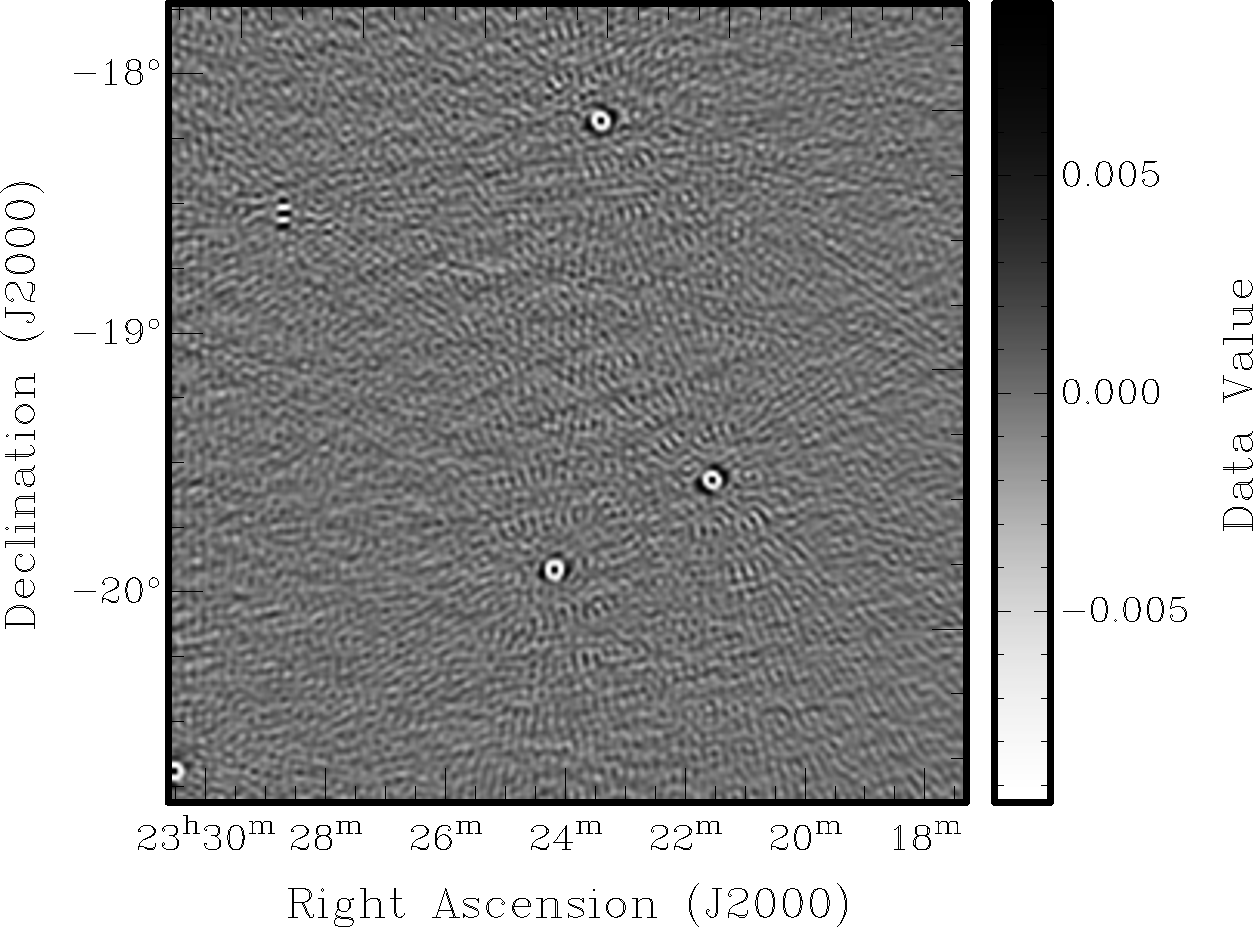
\includegraphics[height=5cm]{img/residual-casa}\hspace{1cm}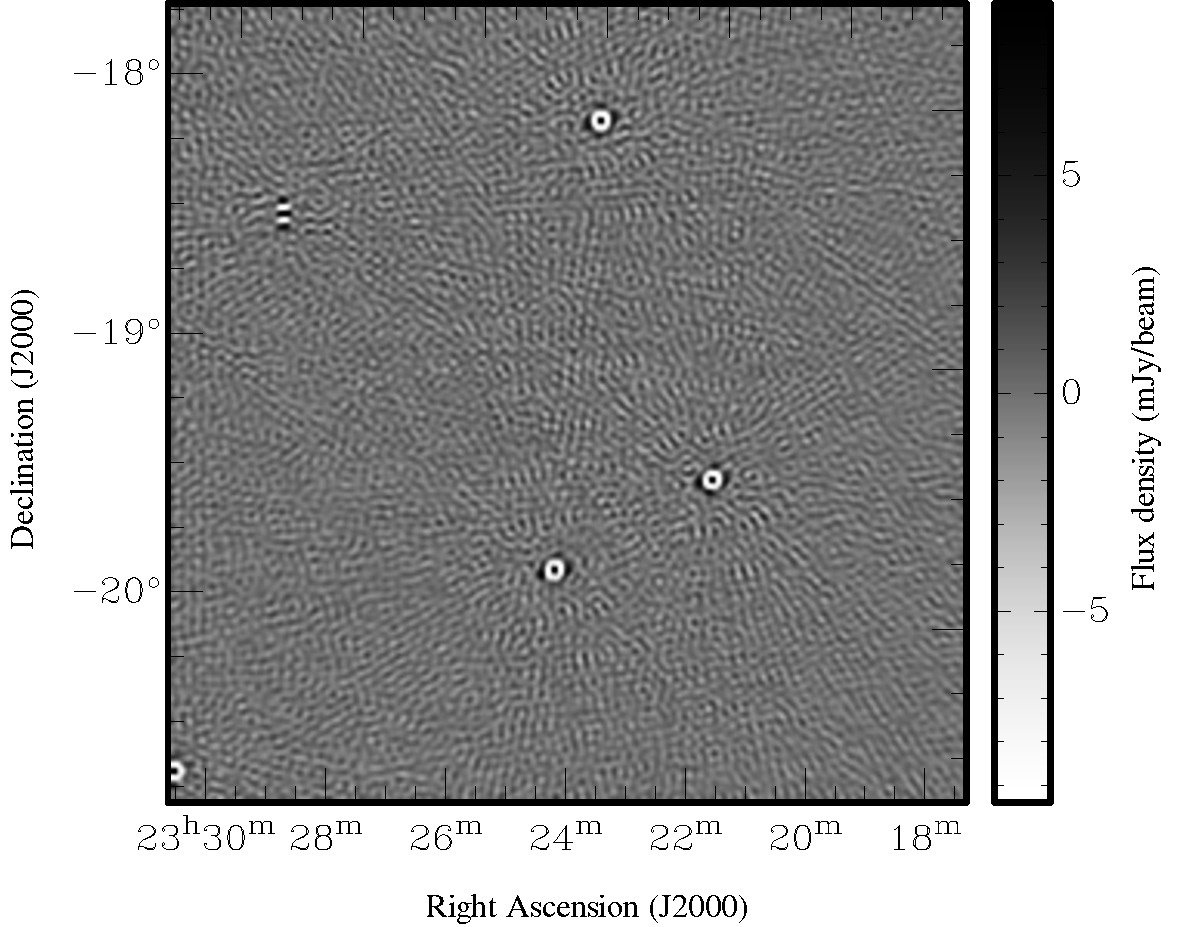
\includegraphics[height=5cm]{img/residual-wsclean}
\caption{Residual images after Cotton-Schwab cleaning of a simulated 10\degree-zenith angle MWA observation using CASA (left) and WSClean (right), using similar inversion and cleaning parameters. The panels show a small part of the full images. The full field contains 100 simulated sources over 20\degree. Sources in the image produced with CASA are slightly less accurately subtracted, leading to a residual noise level of 1.07 mJy and some visible artefacts, whereas WSClean reaches 0.90 mJy. Since the effect is stronger away from the phase centre, it is likely that this is caused by the finite size of the w-kernels used in w-projection, which leads to inaccuracies.}
\label{fig:residuals}
\end{center}
\end{figure*}

To asses the accuracy of WSClean and CASA, we have simulated a MWA observation without system noise, but with hundred sources of 1~Jy in a 20\degree diameter area. A unitary primary beam is assumed. We imaged the simulated set both with WSClean and CASA, using Cotton-Schwab cleaning to a threshold of 10~mJy. The two imagers calculate slightly different restoring (synthesized) beams, hence to avoid bias the restoring beams are fixed. Other imaging parameters are given in Table~\ref{tbl:default-parameters}. The Aegean program \citep{aegean-hancock-2012} is used to perform source detection on the produced images. Sidelobe noise of the residual 10~mJy source structures triggers a few false detections. These are ignored.

Table~\ref{tbl:accuracy-measurements} lists the measured standard errors of the source brightnesses as detected by Aegean and the RMS in the residual image. In all tests, WSClean performs slightly more accurate. At zenith, CASA produces a residual RMS twice as high as WSClean. This is caused by the fact that we keep the number of w-projection planes in w-projection equal to the number of w-layers in w-stacking, resulting in only 12 $w$-planes at zenith. This evidently has a stronger effect on the w-projection algorithm. However, the computational performance of the w-projection algorithm is hardly affected by the number of w-projection planes, and in practical situations one would always use more w-projection planes\footnote{In the zenith case CASA actually issues a warning to use more $w$-projection planes.}. When 128 w-projection planes are used in CASA, its residual RMS is equal to WSClean with 12 $w$-layers. We do not know why this parameter needs to be higher in CASA to reach the same RMS. In theory it should be enough, since Eq.~\eqref{eq:nwlayers-bound} results in $N_\textrm{wlayers}\gg 6$ for the top-left image pixel that is 26\degree away from the centre, while the sources are all within 10\degree. Also unexpected is that the source flux density becomes worse by increasing the number of planes. For WSClean both values stay approximately the same when the number of $w$-layers is increased.

In the $\textrm{ZA}=10\degree$ case, CASA is slightly less accurate. We have noticed this consistently at higher zenith angles, and it can actually be observed in the produced images, as shown in Fig.~\ref{fig:residuals}. TODO the following might be caused by a bug; check: We have also made an image with the technique of recentring a zenith phase-centred visibility set, as described in Sect.~\ref{sec:snapshot-imaging}. Its accuracy is lower compared to the normal projection. This is due to the fact that the sources are further away from the phase centre, and sources have therefore on average higher $(l,m)$-values, thereby increasing the average $w$-correction. Nevertheless, the reprojection technique needs on average fewer $w$-layers to reach the same level of accuracy.

WSClean is faster in all tested cases. WSClean and CASA determine a different next major iteration threshold. CASA performs 5 major iterations at zenith and 8 at 10\degree angle, while WSClean always performs 5 major iterations. Major iterations are dominating the computing time. We will look more closely at the difference in performance in the next section.

Many parameters affect the accuracy more than the observed differences between the methods. These include the number of major iterations, $w$-planes/layers, restoring beam, image size, weighting, kernel size and grid oversampling. Therefore, the differences in accuracy are not very significant. The results do show that synthesis imaging using common imaging parameters results in an approximate flux-density standard error of at least $\sim1\%$.

\begin{figure*}%
\begin{subfigure}{.36\linewidth}%
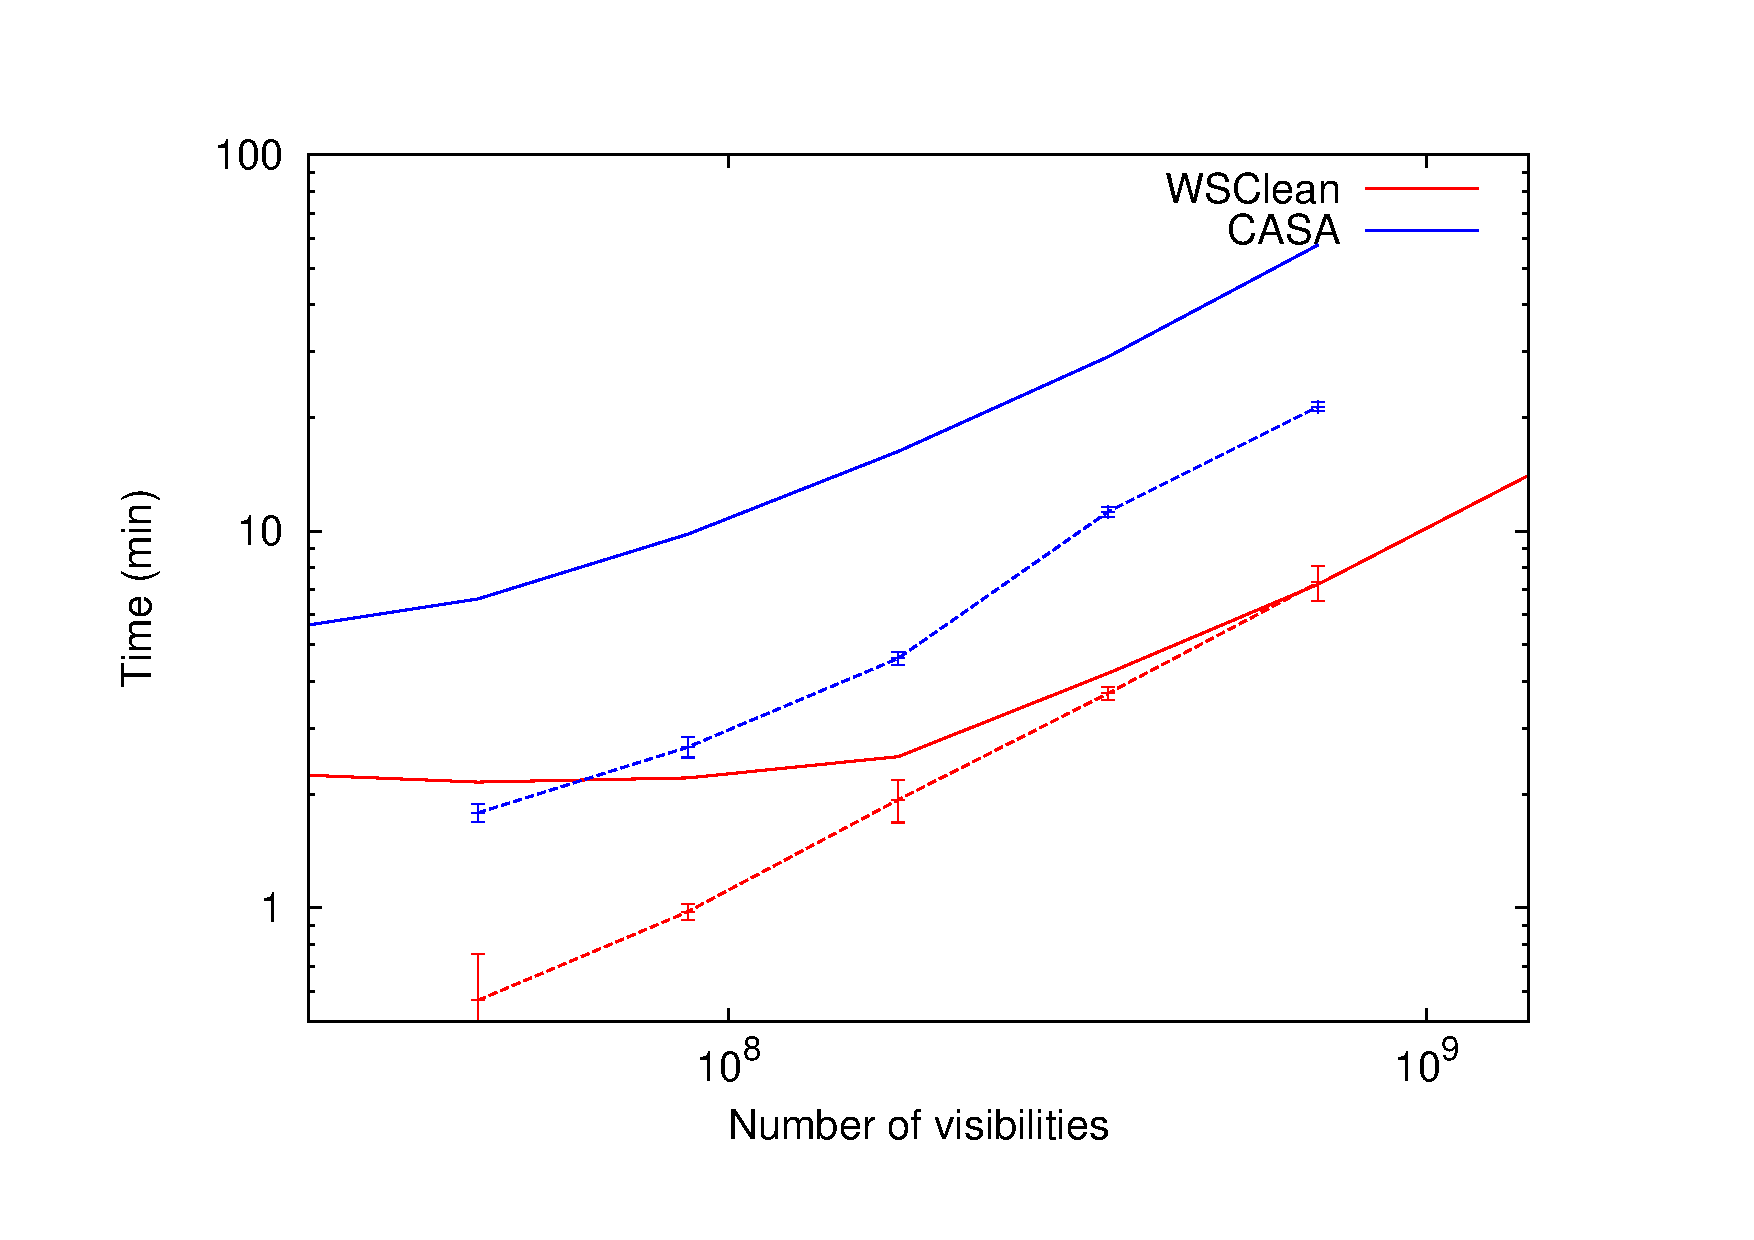
\includegraphics[width=\linewidth]{img/benchmark-nsamples/nsamples}%
\caption{}\label{fig:timing-nsamples}%
\end{subfigure}%
\begin{subfigure}{.36\linewidth}%
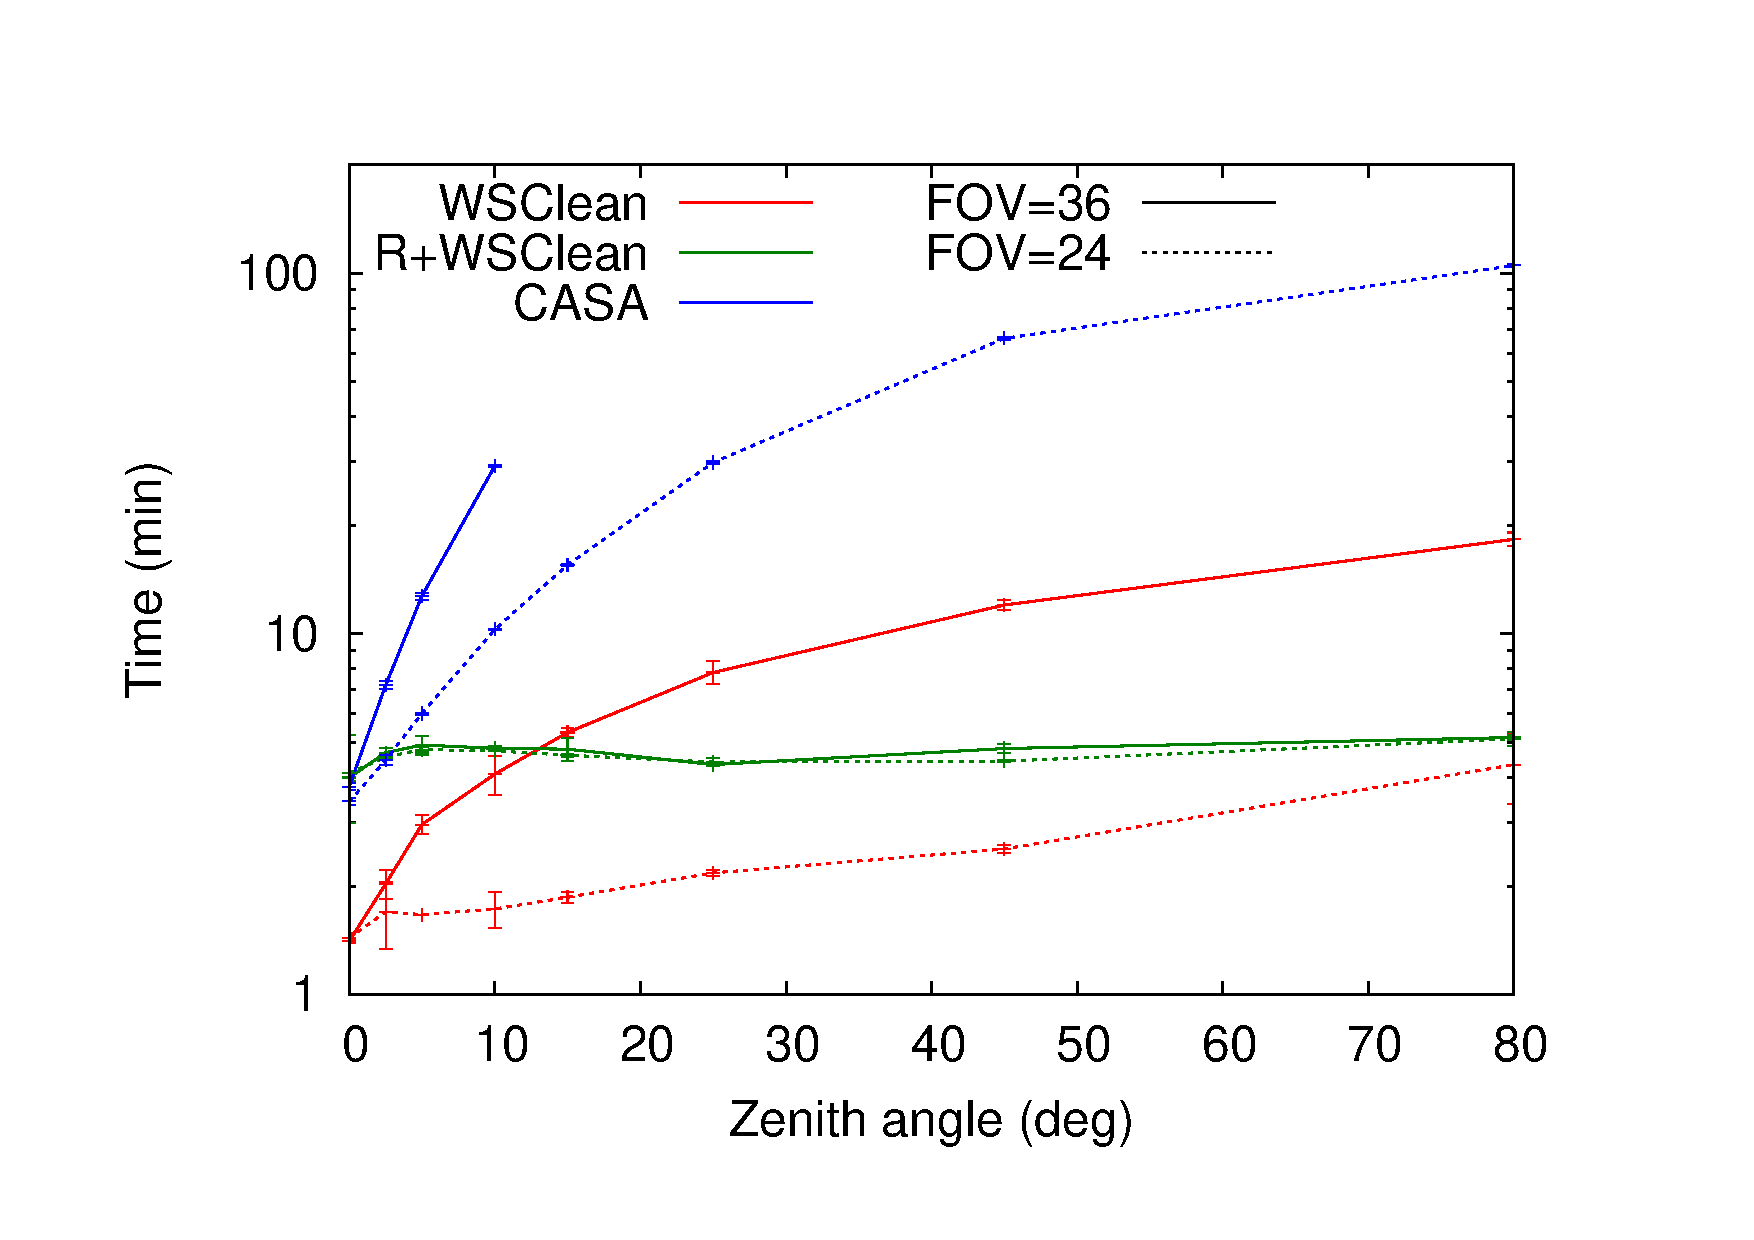
\includegraphics[width=\linewidth]{img/benchmark-zenith-angle/za}%
\caption{}\label{fig:timing-zenith-angle}%
\end{subfigure}\\
\begin{subfigure}{.36\linewidth}%
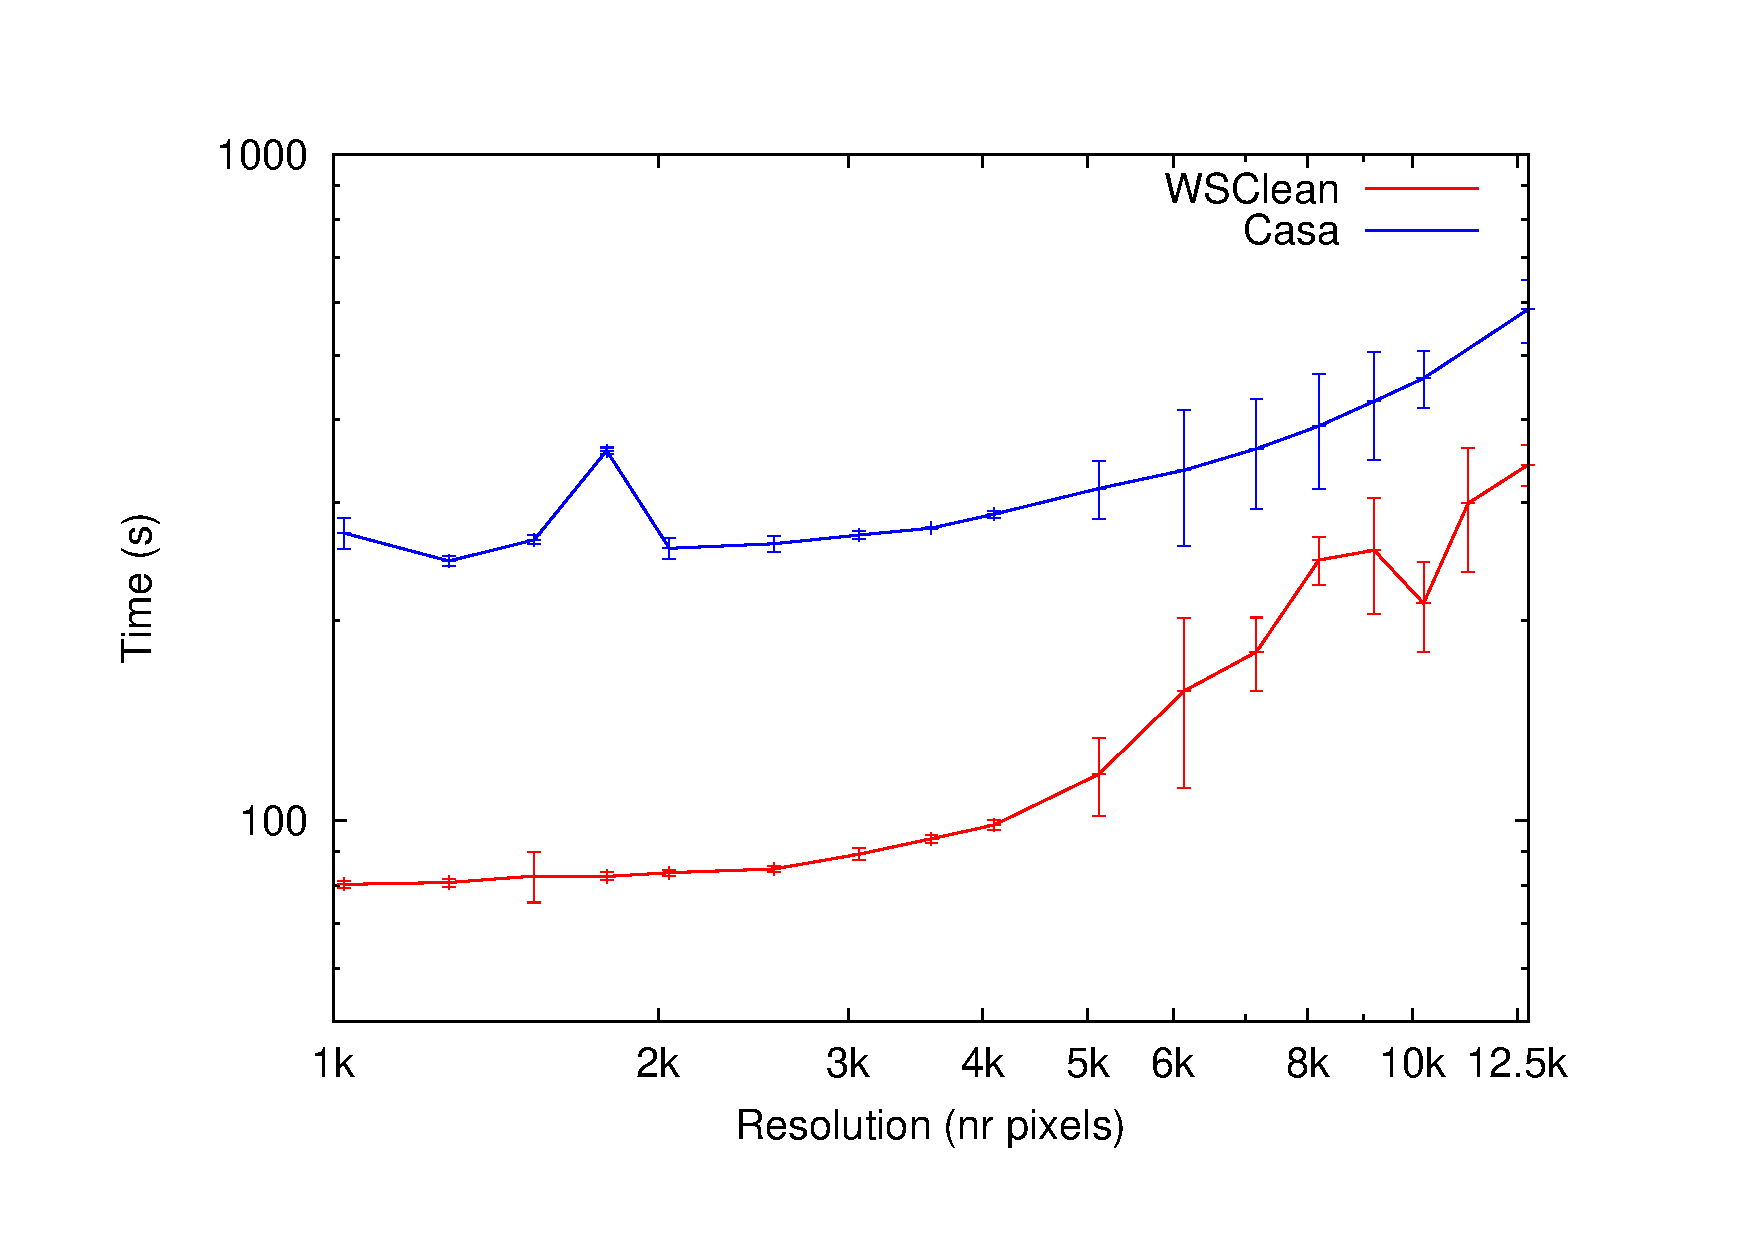
\includegraphics[width=\linewidth]{img/benchmark-resolution/resolution}
\caption{}\label{fig:timing-resolution}%
\end{subfigure}%
\hspace{-.05\linewidth}\begin{subfigure}{.36\linewidth}%
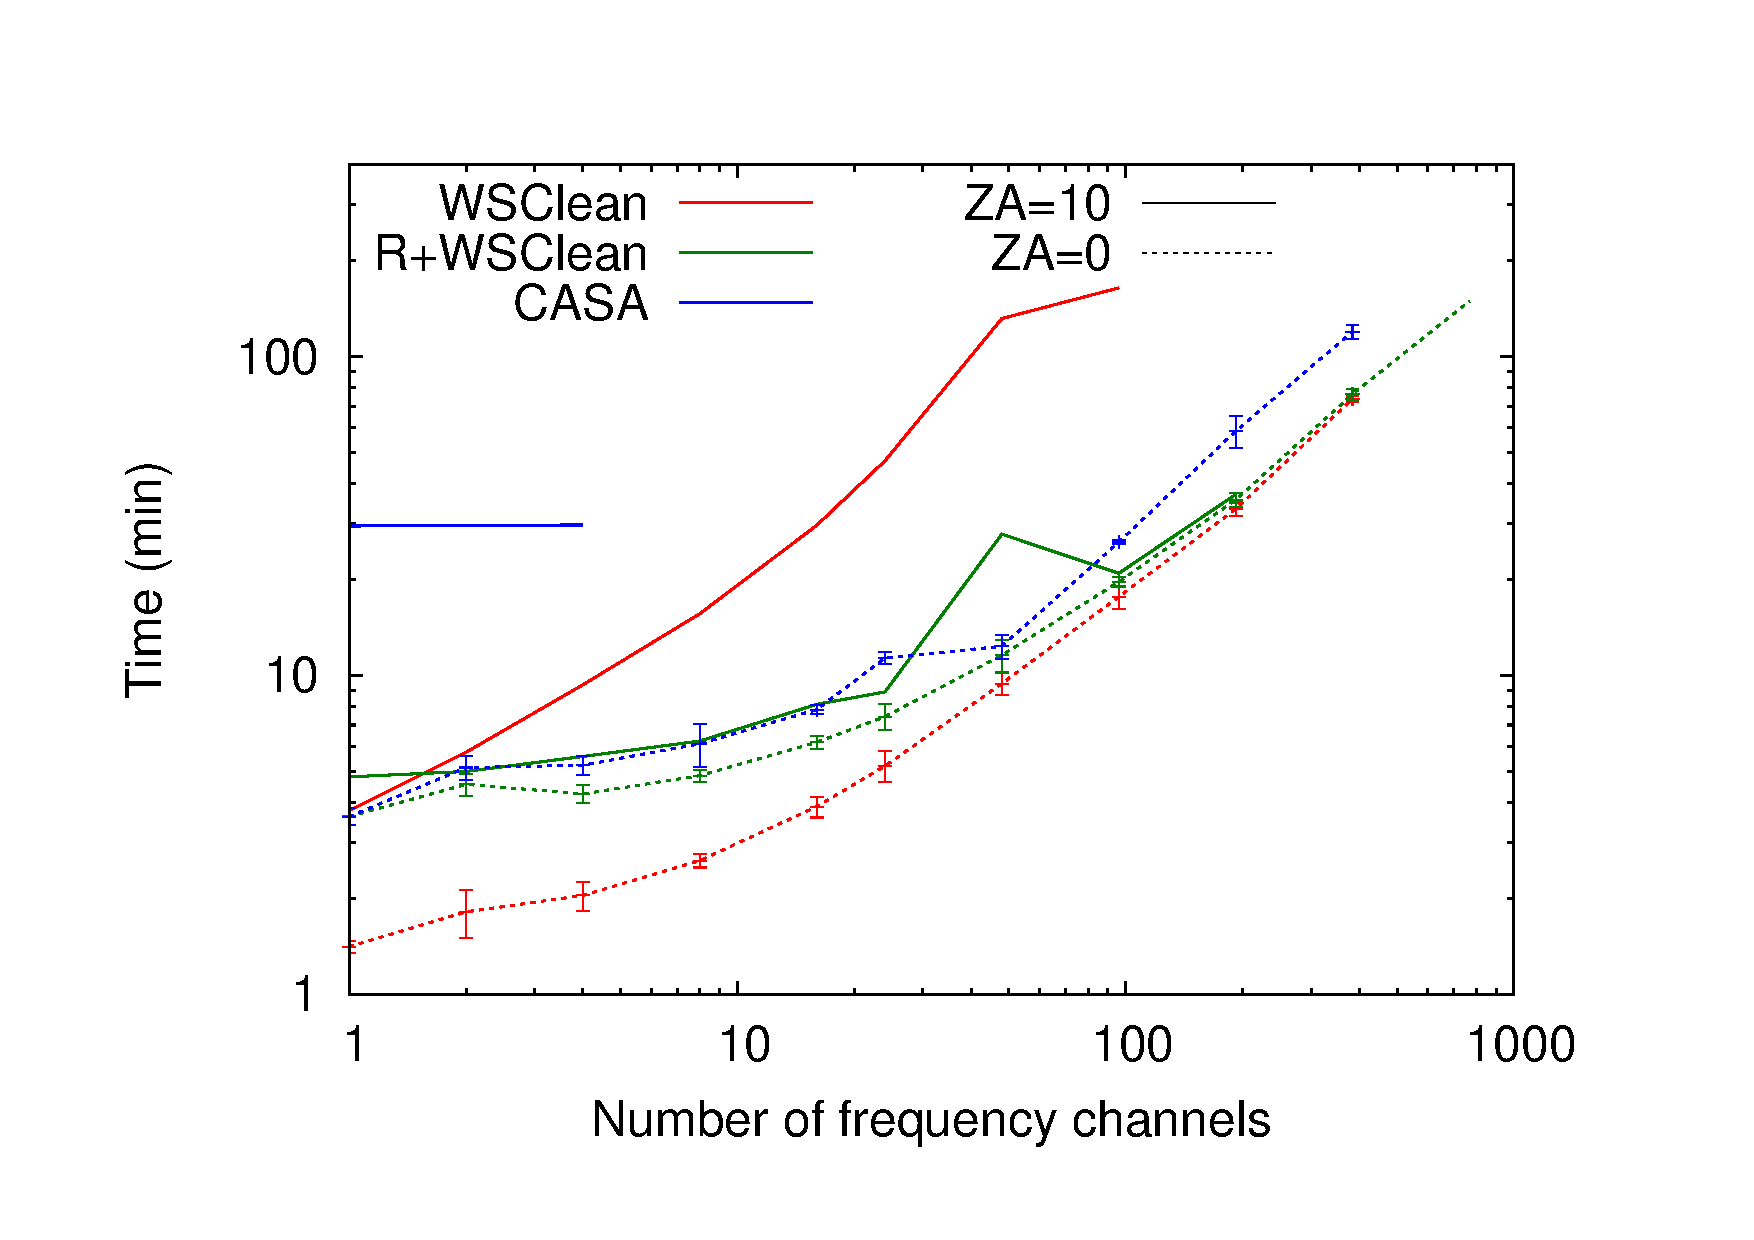
\includegraphics[width=\linewidth]{img/benchmark-channels/channels}
\caption{}\label{fig:timing-channels}%
\end{subfigure}%
\hspace{-.05\linewidth}\begin{subfigure}{.36\linewidth}%
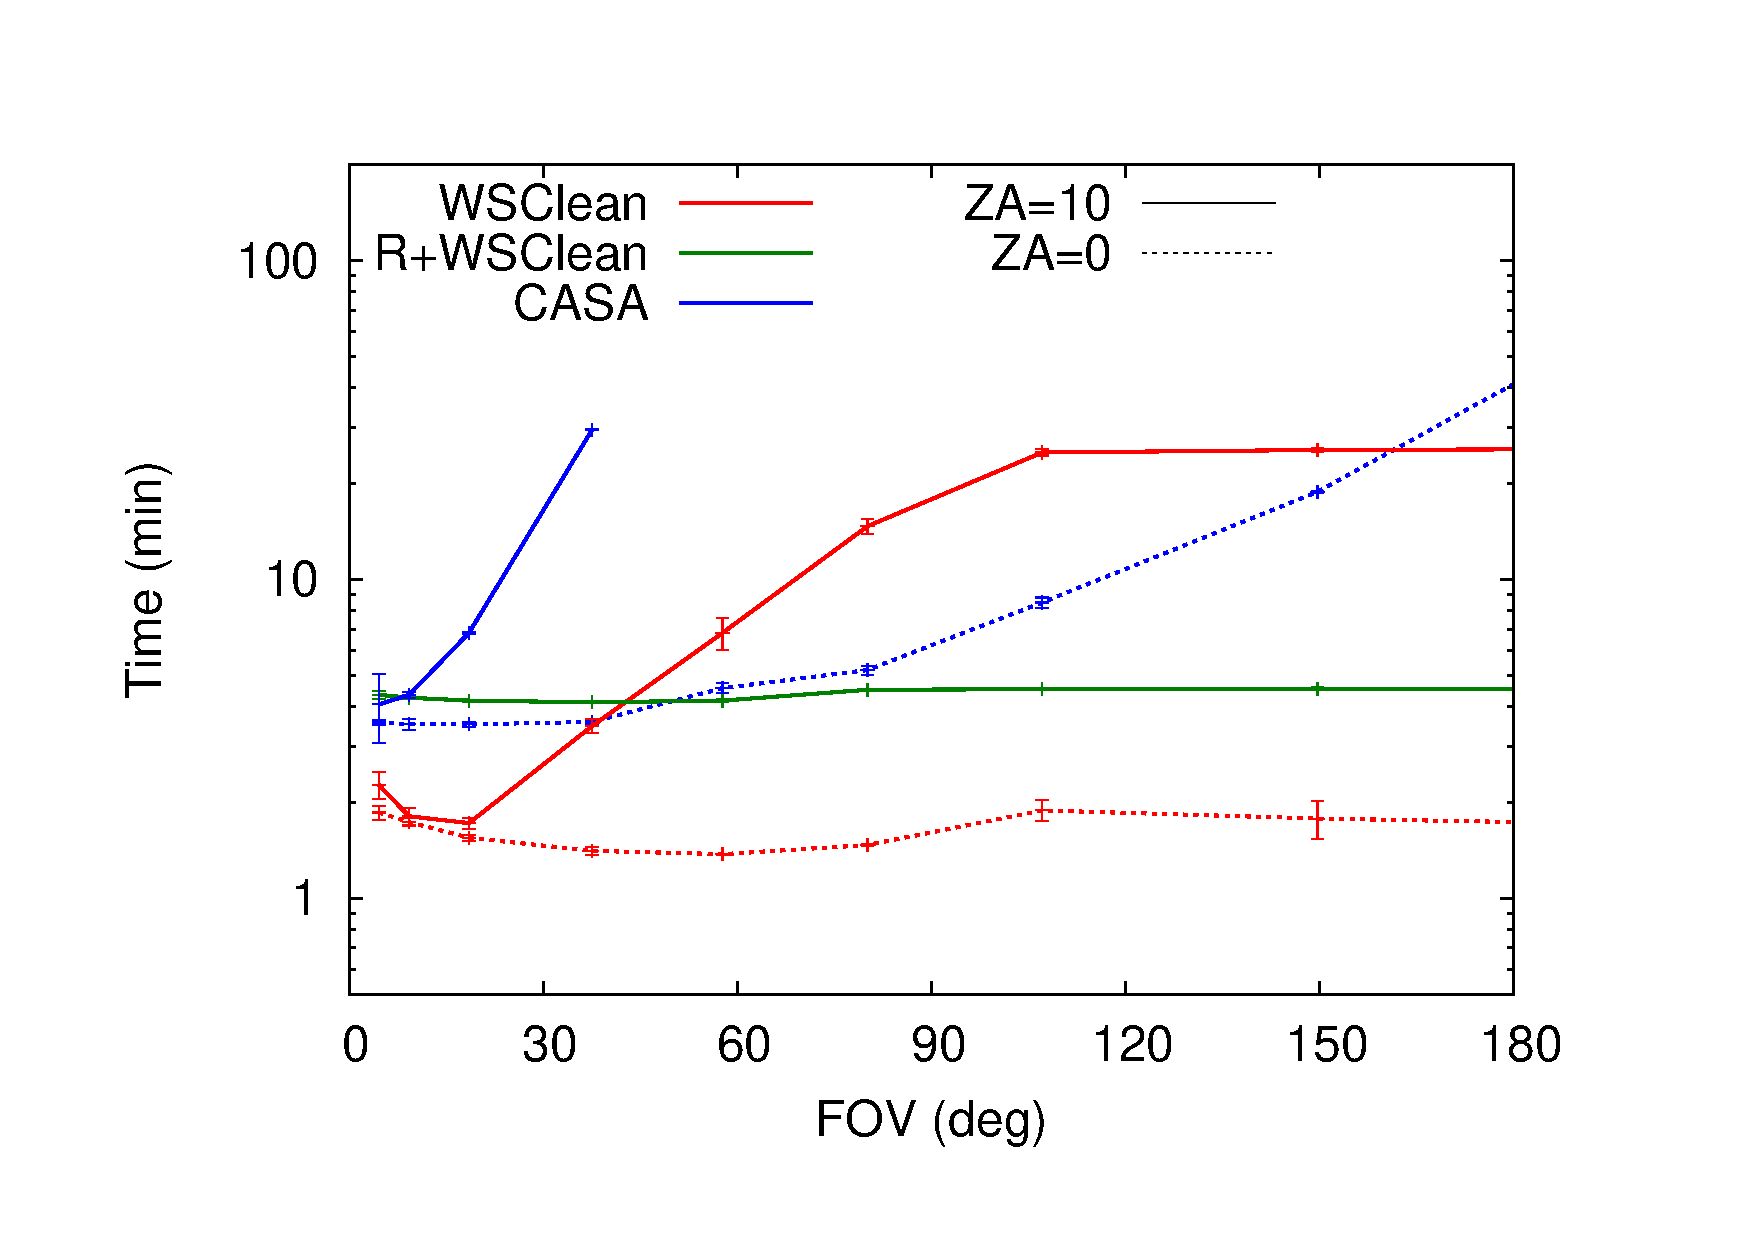
\includegraphics[width=\linewidth]{img/benchmark-fov/fov}
\caption{}
\label{fig:timing-fov}
\end{subfigure}%
\caption{Imaging performance as a function of several configuration parameters. Error bars show 5$\sigma$ level. }\label{fig:timings}
\end{figure*}

\subsection{Performance analysis}

We measured the performance of the imagers using several MWA data sets. Each specific configuration is run 5 times and standard deviations are calculated. The variations between runs is typically a few seconds. In each benchmark, the wall-clock time is measured that is required to produce the synthesized point-spread function and the image itself. No cleaning or prediction was performed. The results are given in Fig.~\ref{fig:timings}.

Panel~\ref{fig:timing-nsamples} shows the dependency on the size of the visibility set. Results for imaging at zenith and 10\degree zenith angle (ZA) are shown. The size of the visibility set was varied by changing the time resolution, which affects the number of visibilities to be gridded without changing the maximum $w$-value. For larger sets, both methods show a linear time dependency on the number of visibilities. This implies that gridding or reading dominates the cost. In that situation, the $w$-stacking implementation is 7.9 times faster at $\textrm{ZA}=10\degree$ and 2.6 times faster at $\textrm{ZA}=0\degree$. With small data volumes, the FFTs start to dominate the cost. This is visible from Fig.~\ref{fig:timing-nsamples} by the flattening towards the left. At that point, WSClean is in both cases approximately 3 times faster. At zenith, the two methods are expected to perform almost identical. The factor of 2-3 difference in Fig.~\ref{fig:timing-nsamples} could be due to different choices in optimizations.

In Panel~\ref{fig:timing-zenith-angle}, the computational cost as function of zenith angle is plotted. It shows that, as expected from \S\ref{sec:time-complexity}, the $w$-projection algorithm is more affected by the increased $w$-values, leading to differences of more than an order of magnitude at zenith angles of $\gtrapprox 20$\degree. Additionally, at higher zenith angles, the $w$-kernels become too large to be able to make images of 3072 pixels or larger. Using the recentering technique to decrease the $w$-values makes the computational cost approximately constant. However, the additional time required to rephase and regrid the measurement set makes it only worthwhile for images $\ge3072$ pixels and $\textrm{ZA}\ge15\degree$. TODO: this is quite heavily depending on the speed of \texttt{chgcentre}, and that might still be improvable...

In Panel~\ref{fig:timing-resolution}, the number of pixels in the image is changed without changing the field of view. The performance of $w$-stacking is more affected by the size of the image, but is still significantly faster in making 12.8K images at 10\degree ZA than $w$-projection. 

Panel~\ref{fig:timing-channels} shows performance versus the output frequency resolution. The cost of imaging at multiple frequencies is the cost of making an images times the number of frequencies. However, each separate imaging contains a part of the total number of visibilities. As shown before, FFTs become the dominant cost for small visibility sets, and performance and number of frequency images therefore have a linear relation, which is clearly visible from the plot.

TODO: for fairness, also check making 4 polarization images.

\subsection{Derivation of computing cost formulae}
Based on the expected cost terms described in Sec.~\ref{sec:time-complexity}, we derive analytical functions for the CASA and WSClean measurements using least-squares fitting. Several functions with different free parameters were tested, and formulae with minimum amount of parameters are selected that still follow the trend of the measurements and have reasonably small errors. The measurements are weighted with the inverse standard deviation. The single outlying measurement of CASA in Fig.~\ref{fig:timing-nsamples} is removed.

For WSClean's time cost $t_\textrm{WSClean}$ we find 
\begin{align}\notag
t_\textrm{WSClean}& (w_e,N_\textrm{vis},N_\textrm{freq},N_\textrm{pix}) = \\ \notag
& 0.000326 N_\textrm{pix}^2 \log N_\textrm{pix} (w_e + 0.000212) +\\
\label{eq:wsclean-computing-cost}%
& 0.252 N_\textrm{vis} - 7.64
\end{align}
and for CASA we find
\begin{equation}
t_\textrm{CASA}(w_e,N_\textrm{vis},N_\textrm{freq},N_\textrm{pix}) = .
\label{eq:casa-computing-cost}%
\end{equation}
Parameter $w_e$ is the maximum $w$ value and is estimated with
\begin{equation}
 w_e = \frac{\max |\mathbf{x}| \sin za + \max z \cos za}{\lambda \max |\mathbf{x}|} \left(1.0 - \cos(\frac{1}{2}\textrm{FOV})\right),
\end{equation}
where $\max |\mathbf{x}|$ is the maximum baseline length, $\max z$ is the maximum height difference between antennas and $\lambda$ is the wavelength.

TODO: actually, $w_e$ should not be normalized by baseline length $\max z$: fix in fits too.

TODO: derive function for $t_\textrm{CASA} = t_\textrm{WSClean}$.

It is possible to combine the $w$-projection and $w$-stacking algorithms by gridding on several $w$-layers to which the large $w$-terms are corrected after the FFT, and using a $w$-correcting kernel for making small $w$-corrections, thereby projecting them on the nearest $w$-layer. This allows using small $w$-kernels and limits at the same time the number of FFTs and required memory. The AWImager has been applied like this, which let to better results compared to $w$-projection without $w$-stacking \citep{awimager-2013}. For this scenario, Eq.~\eqref{eq:casa-computing-cost} can be used to determine the optimal number of $w$-layers, or more general the optimal distance between layers, by assuming that the cost of calculating a single $w$-layer equals the cost of imaging the data set with correspondingly smaller $w_e$ value and smaller $N_\textrm{vis}$. If $\Delta w$ is the distance between $w$-layers, then 
\begin{equation}
t(\Delta w) = \frac{w_e}{\Delta w} t_\textrm{CASA}(w'_e,N'_\textrm{vis},N_\textrm{freq},N_\textrm{pix}),
\end{equation}
with $N'_\textrm{vis} = \frac{N_\textrm{vis}\Delta w}{w_e}$ and $w'_e = \Delta w$.

\section{Application of WSClean to the MWA}
For technical reasons, the MWA correlator splits observations in data products of typically a few minutes. This simplifies $w$-snapshot imaging, which can be done by phase rotating each snapshot to zenith with a possibly additional phase-centre shift. 

TODO: calculate when to use w-snapshots
TODO: calculate optimum splitting time?

\subsection{Beam correction}
Because the MWA consists of fixed, beamformed dipole antennas, the voltage beam of a MWA tile is described by a complex, non-diagonal Jones matrix. Alternatively, Mueller matrices can be used as well, but in general these result in more computations \citep{revisiting-me-i}. When assuming all individual antennas of the tiles are working properly, all tiles have the same beam. The beam can then be corrected in image space for all tiles at once with
\begin{equation}\label{eq:beam-correction}
 I(l, m) = J(l,m)^{-1} I'(l, m) \left(J(l,m)^*\right)^{-1},
\end{equation}
where each term is a $2\times2$ complex matrices, with $J$ the voltage beam and $^*$ denoting the conjugate transpose. Because $J$ is complex and non-diagonal, all 4 combinations of the cross-correlated polarizations $p$ and $q$\footnote{The instrumental polarizations of the MWA are often referred to as $X$ and $Y$ because many software treats the two polarizations as such. However, this is not correct because $X$ is officially defined as being parallel to the celestial equator.} including the imaginary part of the $pq$ and $qp$ are required to calculate any of the Stokes parameters. The $pp$ and $qq$ have no imaginary part due to the $uv$-symmetry. To make proper MWA beam correction possible, WSClean can output real valued $pp$, $pq$, $qp$, $qq$ images and imaginary $pq$ and $qp$ images. Each polarization requires a separate run of the $w$-stacking algorithm. Once these six images are created, a separate program is used to perform the correction of Eq.~\eqref{eq:beam-correction}. This method avoids expensive beam-correcting kernels during gridding, but only works because all tiles have the same beam. To apply the same method on heterogeneous arrays such as LOFAR, each set of correlations with a different combination of station beams will have to be imaged separately, which will increase the cost of the algorithm. The AWImager uses an intermediate method, and corrects a common dipole factor in image space and the phased-array beam factor in $uv$-space, which allows the gridding kernel to be smaller compared to correcting both in $uv$-space \citep{awimager-2013}.

\section{Discussion} \label{sec:discussion}
WSClean has been build out of necessacity to be able to make images with the MWA, because no 

TODO: describe hybrid between w-stacking, w-projection and w-snapshots (if not yet discussed in Cornwell's papers)

TODO: discuss at what is the optimal time to split measurement sets into when using recentering technique.

TODO: A-projection makes the psf more invariant: therefore, truely ``joined'' deconvolution might be more accurate.

TODO: discuss low w-values means less-direction-invariant PSF.

\section*{Acknowledgments}
...
\appendix

\section{Optimal gridding kernel size} \label{sec:gridding-appendix}
\begin{figure}
\begin{center}
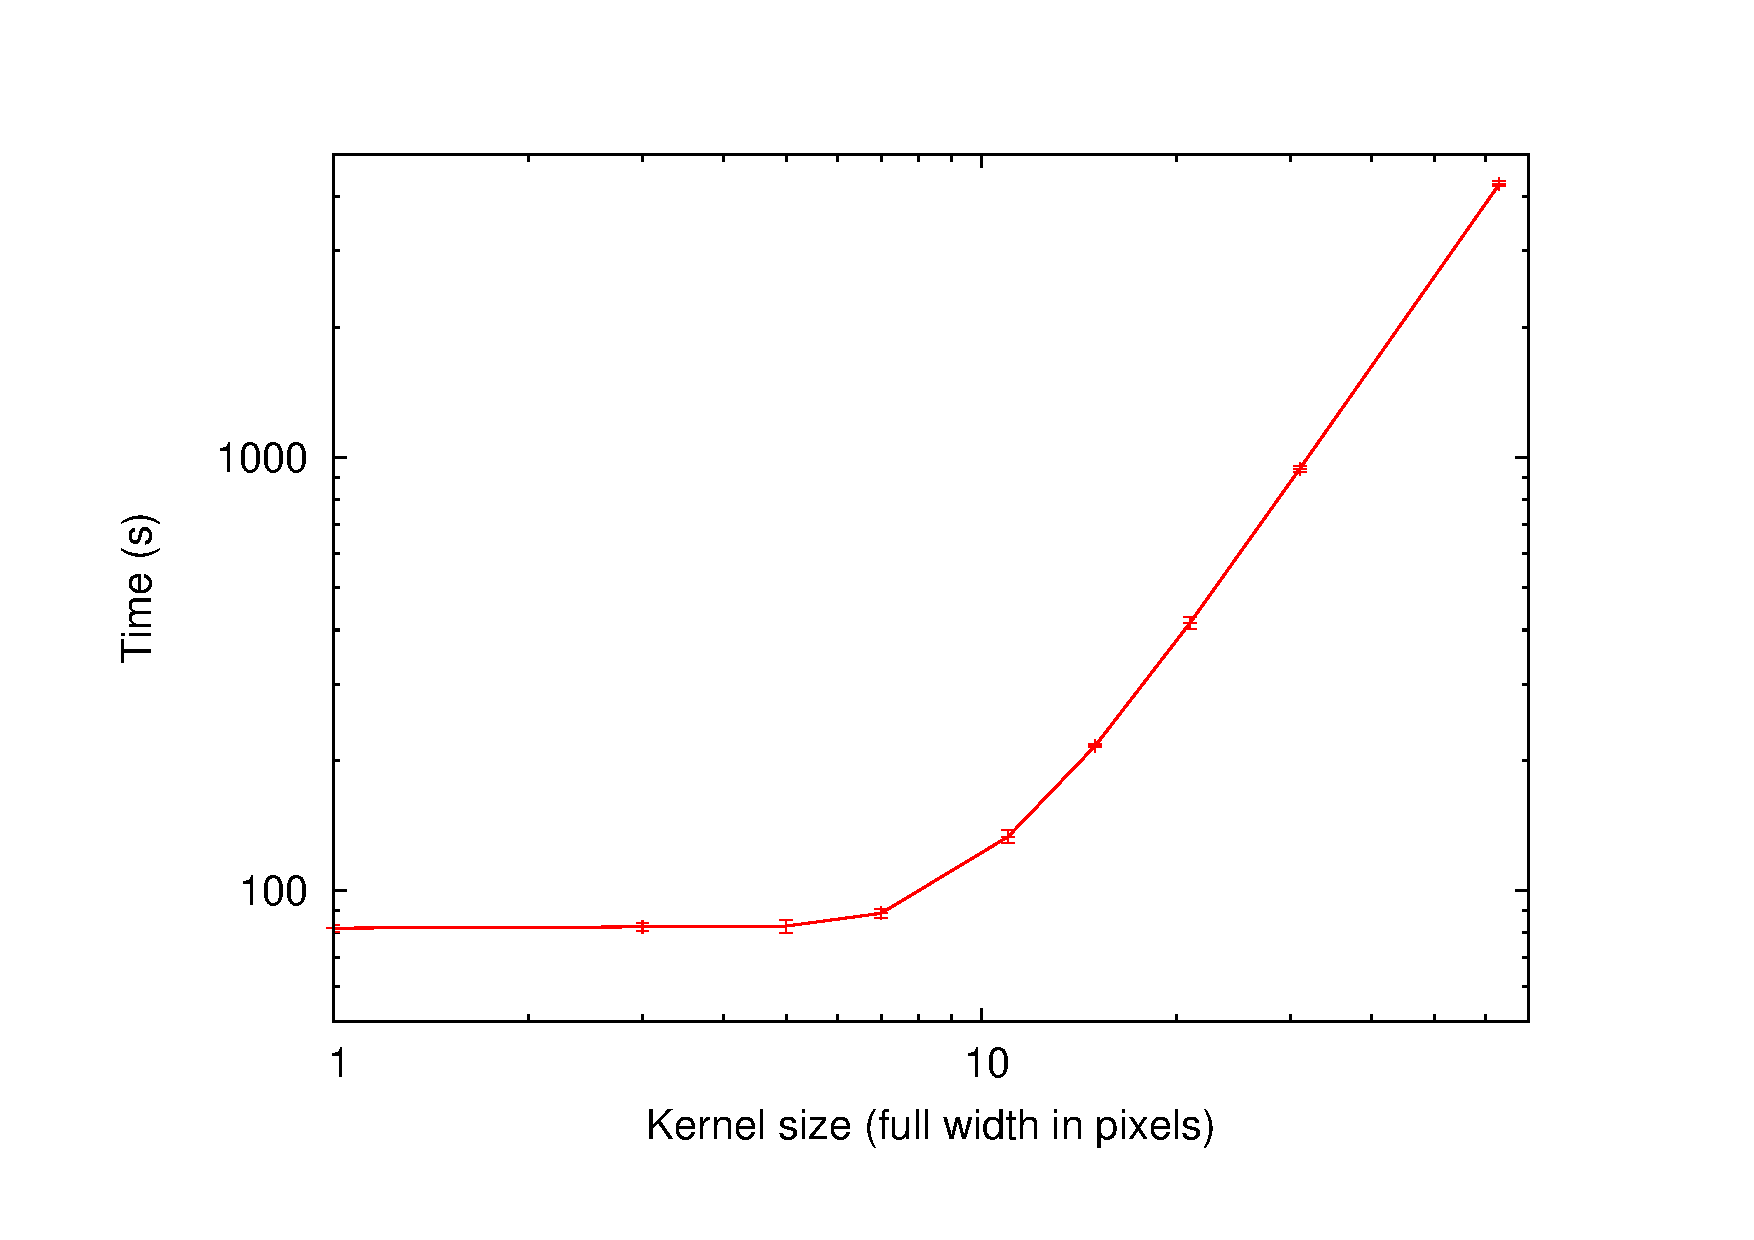
\includegraphics[width=8cm]{img/benchmark-kernelsize/kernel}
\caption{Effect of antialiasing kernel size on performance.}
\label{fig:timing-kernelsize}
\end{center}
\end{figure}
As discussed in \S\ref{sec:gridding}, WSClean uses a Kaiser-Bessel window against aliasing. The type of window function has no effect on the gridding performance, but the size of the kernel affects gridding performance quadratically. Fig.~\ref{fig:timing-kernelsize} shows that this quadratic relation becomes significant for kernel sizes $\gtrapprox 10$. Decreasing the kernel size to values below $7$ has little effect on performance, because for small kernels the visibility-reading rate is lower than the gridding rate. We have not noticed much benefit of larger kernels except in rare cases where a bright source lies just outside the imaged field of view. Therefore, WSClean uses a default of 7 pixels for the gridding kernel. It can be increased when necessary. Of course, different hardware might give slightly different results because of different reading and calculation performance.

% To make Dutch ``tussenvoegsels'' work correctly in Latex such as ``de Bruyn'', we use this command
% In bibliography, it should be written with lowercase, as in ``de Bruyn''
\DeclareRobustCommand{\TUSSEN}[3]{#3}

\bibliographystyle{mn2e}
\bibliography{references}

\label{lastpage}

\end{document}
